\chapter{Implementácia prostredia}
Každý robot má vlastný program, užívateľom definovaný, podľa ktorého sa správa. Tento program sa z hľadiska jednotlivého robota skladá z postupnosti základných inštrukcií (detailnejšie vysvetlené nižšie). Je potrebné zaistiť spravodlivosť pri vykonávaní programu. Robot totiž môže počítať s vlastnými premennými, na ktore nepotrebuje dáta bojiska. Zaistenie spravodlvosti v tomto prípade teda znamená, aby ten robot, ktorý počítal dlho bez toho, aby vykonal nejakú akciu súvisejúcu s bojiskom, prišiel na radu s ťahom o niečo neskôr ako robot, ktorý takúto akciu vykoná okamžite. Toto je splnené tým, že každá inštrukcia je penalizovaná, preto sa najskôr budeme zaoberať penalizáciou a nie samotným priebehom.
\section{Priebeh penalizácie za inštrukciu}
\begin{definicia}
Tick je jednotka virtuálneho času sveta. Timeout je počet tickov,ktoré má robot k dispozícii na premýšľanie a tento čas (ďalej nazývaný timeout) nesmie prekročiť.
\end{definicia}

\begin{definicia}
Penalizáciou za inštrukciu nazývam počet tikov, ktoré robot stratí, ak inštrukciu vykoná. Pre rôzne inštrukcie môže byť rôzna.
\end{definicia}

\begin{definicia}
Programom robota sa nazýva postupnosť inštrukcií, ProgramPointer je ukazateľ na inštrukciu v programe. Druhy inštrukcií a ich vplyv na svet je popísay v \ref{TODO}.
\end{definicia}

Nech je na rade robot R. V tomto okamihu začne R vykonávať inštrukciu, na ktorý práve ukazuje jeho ProgramPointer. Ako je naznačené na \ref{thinking}, robot pokračuje vo vykonávaní inštrukcií až kým nenarazí na takú, ktorá interaguje s bojiskom. Výsledok takejto inštrukcie nie je možné zistiť z dostupných informácií a teda je nutné o ďalšie data požiadať bojisko. Podľa veľkosti penalizovania sa potom R zaradí do plánovaných objektov, viz \ref{timeline}. Dĺžka tejto akcie sa ale pre rovnaký počet inštrukcií pre dvoch rôznych botov môže a typicky bude líšiť. Je to spôsobené tým, že každá inštrukcia môže mať rozdielnu penalizáciu za vykonanie. Napríklad samostatné vykonanie inštrukcie 'step' musí byť niekoľko krát rýchlejšie ako povedzme inštrukcia, ktorá naloaduje hodnotu premennej, obzvlášť ak táto premenná už dlho loadovaná nebola. Ďalej inštrukcia, ktorá zavolá užívateľom definovanú funkciu, zaberie viac procerového času vzhladom na to, čo musí spraviť so zásobníkom robota, a preto je táto skutočnosť zohľadnená. Podobne napríklad inštrukcie pre násobenie a delenie su zlošitejšie ako prosté sčitanie a preto sú viac penalizované. Penalizácia prebieha podľa tabuľky \ref{penal}, v ktorej používam nasledujúce funkcie:
\begin{itemize}
\item SizeOfJump: počet inštrukcií medzi miestom skoku a miestom určenia
\item SizeOfFunction: počet inštrukcií vo funkcii
\item SizeOfCleaned: počet premených, ktoré sa stali odchodom z bloku príkazov neplatnými
\item LastLoaded: počet tickov, ktoré ubehli od posledného loadovania
\end{itemize}
\begin{table}[ht]
\centering
\caption{Výpočet penalizácie inštrukcie}
\begin{tabular}{|c | c |}
\hline
Inštrukcia & Penalizácia \\
\hline
Jump & SizeOfJump\\
Store & 1 \\
Plus & 1 \\
Minus & 1 \\
Multiply & 2 \\
Divide & 4 \\
Less & 1 \\
LessEqual & 2 \\ %kontroluje sa aj real/integer!
Call &  SizeOfFunction \\
StartBlock & 0 \\ %iba zvysi aktuane zanorenie
EndBlock &  SizeOfCleaned \\
Load & LastLoaded \\
Label & 0 \\
Return & 1 \\
\hline
step & 1\\
see & 3\\
shoot & 1\\
turn & 1\\ 
\hline
\end {tabular}
\label{penal}
\end{table}

\begin{figure}
\centering
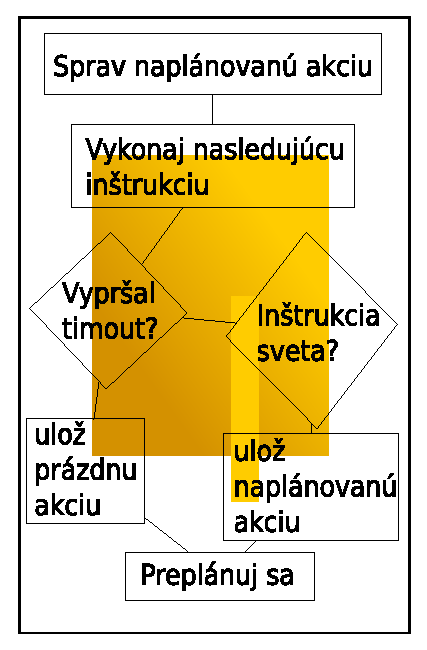
\includegraphics[totalheight=0.2\textheight,width=.2\textwidth]{thinking}
\caption {Priebeh premýšľania u robota}
\label{thinking}
\end{figure}

Robotovi môže týmto spôsobom samozrejme vypršať čas, veľkosť jeho premýšľania dosiahne hodnoty timeout.%TODO ref
V takom prípade, ako je naznačené na obrázku \ref{thinking} sa robot vzdá, preplánuje sa a uvoľní miesto nasledujúcemu objektu. 
\newline
Nech je na rade objekt rôzny of typu 'robot'. Potom tento objekt má konštantnú penalizáciu a jeho program obsahuje iba inštrukcie, ktoré interagujú s bojiskom.Sú rôzne v závislosti na type objektu.

\subsection{Preplánovanie}
Preplánovanie prebieha tým spôsobom, že sa podľa tabuľky \ref{penal} spočíta, koľko času robot prehmrhal na myslenie, presne o toľko sa posunie v pomyselnej casovej osi a zaradí sa vo fronte udalostí za posledného bota s rovnakým časom. To spôsobí to, že robot, ktorý nebol na rade dlhšie, sa dostane k akcií skôr, čo je opäť jedna z podmienok fair-play. Samotné inštrukcie interagujúce s bojiskom  majú jednu z najmenších penalizácií, čo odpovedá tomu, že je to pre bota akoby prirodzená akcia(žodpovedá to skutočnosti,že človek sa obvykle rýchlejšie pohne ako vypoćíta mocninu dvoch) \\
V tomto prípade sa za kľúč, podľa ktorého sa objekty usporadúvajú, považuje čas od začiatku behu hry. Problém ale nastáva v okamihu, keď tento čas pretečie. Vzhľadom na to, že celkový čas simulácie je ukladaný do 64-bitového integeru, je možnosť, že by tento čas pretiekol, krajne neprijateľný, pretože celkový čas by bol vačší ako niekoľko tisíc rokov:)\\
Otázkou zostáva, ako implementovať túto časovú líniu tak, aby celý program nepůsobil trhane, teda aby v okamihu, keď robot rozmýšľa, ostatné objekty, ktoré sú na rade, sa mohli pohybova+t, keďže samotné premýšľanie sa ich nedotýka. Existuje niekoľko možností:
\begin{itemize}
\item Z robotovho programu sa približne odhadne, koľko budei minimálne premýšlať a po tomto čase sa pozrie, či výpočet dobehol. Ak nie, bude musieť čakať, ak áno, pokračuje sa s zozbrazovaním akcií, ktoré sú výsledkom inštrukcií objektov. 
Výhody tohoto prístupu:\begin{itemize}
	\item Plus: Je zachovaná správna postupnosť akcií, to znamená, že nie sú závislé na procesore a jeho súčasnej vyťaženosti.
	\item Minus: Odhad sa můze od skutočnej penalizácie líšiť stovky tickov (napríklad v prípade u podmieneného skoku sa načíta funkcia, ktorá stoji ohromne moc, kým v druhej vetve sa robot okamžite pohne), tým by vznikali nechcené prestoje a simulácia by sa v istých situáciách trhala.
	\end{itemize}
\item Dopredu sa nasimuluje časť priebeh hry a na výstup sa púšťajú už iba výsledky. Výhody a nevýhody:
	\begin{itemize}
	\item Plus: Simulácia sa bude zatrhávať maximálne raz za čas, v okamihu, keď ešte nebudú pripravné data, čo sa 
	\item Minus: na jednoprocesorovych architekturach ma tento spôsob rovnaký efekt ako keď sa súčasne vykresľujú oneskorené výsledky a súčasne poćítajú aktuálne časové línie.
	\end{itemize}
\end{itemize}
Kód robota sa za jeho života nemení. 

\section{Hracia plocha} % z coho sa sklada
Na začiatku hry sa vygeneruje mapa s veľkosťou, ktorú zadá užívateľ, alebo sa načíta už uložená mapa. Táto pozostáva zo voľných políčok a stien. Steny sú rôzneho typu, viz \ref{kap}. Ďalej celú túto konštrukciu nazývam bojisko. V tomto okamihu je hra pripravená na spustenie. V závislosti na veľkosti bojiska sa čaká na odpovedajúce množštvo robotov, ktorí sa zapoja do hry. Toto množstvo je defaultne obmedzené iba zdola. Na zdôvodnenie tohoto rozhodnutia je nutné spomenúť základné vlastnosti programu. 
garantovaný, nastávajú dve možnosti, ako to tom informovať robota:
\begin{itemize}
\item za cieľ by sa simulovalo ľubovoľné políčko, ktoré je mimo mapy. V tomto prípade by robot prinajlepšom cyklicky prehľadával celú mapu, čo je v podstate to isté akoby pozíciu vôbec nepoznal.
\item za cieľ by sa vybralo políčko patriace mape. V tom prípade 
\item Je zabezpečená spravodlivosť pre robotov. To znamená
\end{itemize}

v  že pri neprimarane veľkých mapách bude trvať príliš dlho, než sa roboti vobec  
Nastavenie toho, ze roboti so takto obmedzení, a dá prenastaviť v settings.%TODO rozpisat v+setky menu, +co kde robia
\subsection{Generovanie map}% ako sa generuje, podpora ukladania, zadne zhluky, vyhody, nevyhody, 
\section{Jazyk hry a priebeh hry} %bison, preco
\begin{definicia}
Cieľom určenia robota nazývam políčko na mape sveta, kam sa má robot dostať. Teda ak je pozícia robota rovnaká ako pozícia tohoto cieľu, hra končí. Týchto cieľov môže byť viac. V prípade viacerých cieľových oblastí má užívateľ možnosť zvoliť voľbu \it{Vlastný Exit}, kde sa každému robotomi priradí práve jedna cieľová pozícia a to tá najvzdialenesia od jeho výskytu v mape po začatí hry.
Pod vzdialenosťou rozumiem veľkosť obsahu obdĺžnika v vrcholmi cieľom a výskytom robota. %TODO preco?
\end{definicia}

Samotná hra prebieha tak, že roboti vykonávajú užívateľom definovaný kód až do okamžiku, keď dosiahnu cieľ určenia alebo kým zostane na bojisku maximálne jeden robot. Cieľ môže byť pre každého robota rozdielny a je súčasťou mapy sveta. Hra nie je zabezpečená proti nekonečne dlhotrvajúcim cyklom (napríklad keď každý robot stojí na mieste), predpokladá sa v tomto prípade vstup od uživateľa, ktorým hru prerusí.

\begin{definicia}
Stav robota vzhľadom na svet charakterizuje štvorica: (InstructionPointer IP, Hitpoints HP, VisualMemory vm, Direction direct), kde 
\begin{itemize}
\item InstructionPointer je odkaz do štruktúry programu robota hovoriaci, ktorá inštrukcia je na rade
\item HP je nezáporné celé číslo popisujúce životnosť robota
\item VirtualMemory je štruktúra obsahujúca objekty v zornom poli od posledného volania funkcie 'see()', volanej bez parametrov 
\end{itemize}
Stav robota s ohľadom na inštrukcie, ktore vykonáva, charakterizuje (PointerStack PS, ValueStack VS, Memory m) kde
\begin{itemize}
\item PS zoznam pointerov do štruktúry programu
\item VS je zásobník všetkých naloadovaných hodnôt, parametrov  a návratových adries z funkcií
\item Memory je zoznam všetký doteraz definovaných premenných a funkcií
\end{itemize}
\label{StavRobota}
\end{definicia}

\begin{definicia} 
Pod objektami sveta rozumieme všetky prvky, ktoré svet tvoria a zároveň ho z času na čas menia, t.j. v tomto prípade strely, steny, a samotní roboti. Napríklad strela mení svet tým, že sa pohne alebo narazí, istý druh steny sa môže posunúť a pod.
\end{definicia}
Svet je charakterizovaný dvojicou $< FrontaUdalosti, Bojisko >$, kde FrontaUdalosti je fronta objektov, ktoré sú na rade, aby komunikovali so svetom. Presný spôsob definovania poradia tejto komunikácie je popísaný neskôr. Objekty v tejto fronte sa počas priebehu boja menia, napríklad pribúdajú a zanikajú strely, ktoré sú podla \ref{defobjekty} tiež objektami.

Pre všetky nasledujúc inštrukcie interagujúce so svetom predpokladajme, že svet je v stave $<FrontaUdalosti, Bojisko>$, kde FrontaUdalostí je postupnosť objektov $(robot X, objekt1, objekt2, objekt3,...objektN)$ a Bojisko je dvojrozmerná matica popisujúca, aké objekty sú na akých pozíciach.
Popis jednotlivých inštrukcií a ich vplyv na svet je symbolicky popísaný takto: (bez parameterov, ktoré nemajú vplyv na svet):\\
\newline
step:\begin {itemize}
\item Svet:$ < NewQueue, m.reinsert(X) > $
\item Bot: $ < NewIP, HP, direct> $
\end {itemize}
turnLeft, turnRight \begin{itemize}
\item $Svet:  <NewQueue, m>$
\item $Bot:  < NewIP, Hp, NewDirect)>$
\end{itemize}
turn  \begin{itemize}
\item $Svet:  < NewQueue, m > $
\item $Bot:   < NewIP, Hp, NewDirect)> $
\end {itemize}
see  \begin{itemize}
\item $Svet:  <NewQueue,m> $
\item $ Bot:  < NewIP, Hp, NewDirect)> $
\end {itemize}
shoot \begin {itemize}
\item $ Svet:  < AddQueue, m> $ 
\item $ Bot:  < NewIP, Hp, Direct)>  $
\end {itemize}
\indent
kde NewQueue je \\ $(Objekt_1, Objekt_2, ..., Objekt_K, X, Objekt_{k+1},.., Objekt_N)$, NewIP je nový ukazateľ do programu robota, nie nutn odlišný od predošlého, NewDirect je číslo 1-4 označujúce aktuálne natočenie robota, reinsert je funkcia, ktorá sa pokúsi robotom pohnut v mape, ak sa nedá vyvolá sa ošetrenie kolízií a AddQueue je\\ $(Objekt_1, Objekt_2, ...,Object_{strela},..., Objekt_K, X, Objekt_{k+1},.., Objekt_N)$ (strela bude na rade typicky pred robotom, ktorý j vypustil, pretože ten robot sa preplánuje, ale strela ešte na rade nebola, tak mś vyššiu prioritu.)
Ďalšie inštrukcie vôbec nekomunikujú so svetom, preto sú uvedené oddelene. Tieto inštrukcie robot vykonáva počas svojho premýšľania. Keďze tým robot vobec nepotrebuje vedieť o objektov sveta iných než je on sám, po prevedení takýchto inštrukcií sa meni stav robota podla tabuľky \ref{VnutroBota},kde IP+1 znamená posun v atuálneho pointera v programe robota o jednu inštrukciu ďalej, AddedIP je uloženie aktuálneho pointera na inštrukciu a vyhlásenie iného pointera za aktuálny (typicky začiatok pricedúry alebo funkcie), VariablesAdded je pamať robota rozrastená o premenné danej funkcie alebo procedúry v danom zanorení, ClearVariables je označenie premennych definovaných v tomto bloku za neplatné, LoadByName je uloženie hodnoty volanej premennej na ValueStack, AddedResult je uloženie výsledku aritmetických operácií na ValueStack a DeleteIP je zrušenie aktuálneho pointera na funkciu a obnovenie predchádzajúceho na inštrukiu, pre ktrou bol prerušený. RemoveValue je spracovanie hodnoty zo ValueStacku a teda jej odobranie a odobranie premennej, do ktorej sa priradzuje.

\begin{table}[ht]
\centering
\caption{Vnutorné príkazy robota}
\begin{tabular}{|l|p{5cm}|}
\hline\hline
Inštrukcia & Stav bota po inštrukcii \\
store & $ IP+1,RemoveParameters$\\
aritmeticke+relacne operácie & $IP+1,AddedResult,m$ \\
Call &  $ AddedIP,VS,VariablesAdded$\\
StartBlock & $IP+1,VS,m$\\
EndBlock & $IP+1,VS,ClearVariables$\\
Load & $ IP+1,LoadByName,m$\\
Label & $ IP+1,VS,m$\\
Jump & $ DeleteIP,VS,t$\\
\hline
\end{tabular}
\label{VnutroBota}
\end{table}

\subsection{Vlastnosti stien} % vseobecne oba rozne vlastnosti, ake maju steny, k comu to je
Steny sú objekty sveta, cez ktoré robot nevidí a ktoré môžu napríklad vychýliť dráhu strely. Nie sú však len statické, exituje viacero druhov stien, ktoré budú kominikovať s mapou. Sú to:\\
\begin{itemize}
\item zvláštne políčko Exit, na ktoré sa má robot dostať. Pokiaľ je políčok viac, a nie je difinované inak, robot sa musí dostať do toho najvzdialenejšieho exitu od miesta, kde začínal.
\item MovableWall, touto stenou je možné pohnúť, ak na políčku za za ňou v smere pohybu nič nie je.
\item TrapWall. Táto stena vždy na náhodný počet tikov zmizne a znova sa objaví. V prípade, že sa v okamžiku jej objavenia je na jej políčku nachádza iný objekt, ráta sa to ako kolízia, viz neskôr.%TODO referencia
\item SolidWall, obyčajná stena bez špeciálnych vlastností.
\end {itemize}
Steny sa dajú kombinovať, to znamená, že napríklad východ sa môže pohybovať alebo miznúť. 
\subsection{Viditeľnost robota}
V úvode si užívateľ má možnost nastavit dve premenné, ktoré ovplyvňujú to, ako ďaleko bud robot vidieť. Sú to premenné  'uhol' a 'vzdialenoť'. Tieto premenné sa navzájom ovlyvňujú a teda počet bodov, ktorý sa medzi nich má rozdeliť, je nezávislý na počte bodov u ostatných vlastností robota. Maximálna veľkosť \'vzdialenosti\' je 32, uhol môže byť až $90\,^{\circ}$. Uhol je zadávaný v stupňoch aby sa predišlo načítavanie reálnych hodnôt a tým k strate informácií.
\begin{definicia}
Pod zorným poľom robota rozumieme kruhovú výseč o polomere 'vzdialenosti'.Robot vidí objekt v okamihu, ked vidí stred políčka, na ktorom objekt stojí a úsečka spájajúca tieto dva body nepretína žiadny ďalší objekt.
\end{definicia}
Vzdialenosť a uhol určujú obdĺžnik, ktorý obsahuje presnú polovicu zorného poľa robota.a Tento obdĺžnik môže mať vzhľadom na podmienku o zadávaní vzialenosti a uhla maximálne obsah 32. Pri vytváraní robota sa vygeneruje obdĺžnik a každému políčku sa priradí maska. Nech má obdĺžnik rozmery (x,y) a jeho dolný ľavý vrchol je na pozícií (0,0), čo je v podstate pozícia bota. Táto maska sa potom spočíta tak, že na vygeneruje úsečka spájajúca(0,0) postupne so všetkými stredmi políčok hornom trojuholníku. Každému políčku potom priradíme 32-bitovú masku, kde jedničky sú na pozíciach čísla toho políčka, cez ktoré táto úsečka prechádzala. Druhá polovica je presne symetrická, teda masky tejto polovičky nemusíme počítať zvlášť. Potom na zistenie, ktoré objekt sú viditeľné a ktoré nie, stačí v mape prejst tento obdĺžnik 2x (raz doľava a raz doprava) s počiatočnou maskou nulovou a v prípade, že sa na i-tom políčku zhoduje maska políčka s majou maskou binárne sčítanou s maskou políčka, na to políčko obot vidí. Ak tam je ďalej objekt, nastaví sa v skúšobnej maske na i.tom mieste nula, inak jedna. Ak sa masku nezhodujú, potom robot na toto políčko nevidí a skúšobná maska bude mať na i-tom mieste nulu.
\indent
\subsection{Priebeh výpočtu robota} %co je povolene a ako sa to riesi implementacne
..\\
Zaujímavejšie je to pri volaní funkcie, ktorá má defaultný parameter. Pretože sa predpokladá, že program bude prístupný aj pre obyčaných užívateľov, je možné u funkcie definovať aj explicitnú hodnotu a to nezávisle na poradí parametrov. T.j. explicitné hodnota môže byť zadaná ako prvý a tretí parameter, ale nie ako druhý. Takáto funkcia sa nadefinuje podobne ako v C/C++, napríklad : \\\center $ function distance(integer x=3, integer y=2, integer radius, Location l) $ \\ je funkcia, ktorá bude napr
\subsection{Detekcia zacyklenia}

\section{Vlastnosti robotov}
Výsledok programu, ktorého inštrukcie robot vykonáva, je závislý na konkrétnom type robota. Typ robota je definovaný niekoľkými parametrami, ktoré si bežný užívateľ samostatne na začiatku hry definuje == UholViditelnost, PolomerViditelnosti, Obrana, Hitpoints, TypStrely, VelkostPamate==
\begin{table}[ht]
\caption{Vlastnosti robota}   % title of Table
\centering                          % used for centering table
\begin{tabular}{cl}            % centered columns (4 columns)
%\hline\hline                        %inserts double horizontal lines
Vlastnost & Vplyv \\   % inserts table
%heading
%\hline                              % inserts single horizontal line
polomer viditeľnosti & Robot dokáže na určitú vzdialenosť rozpoznať object, táto vlastnosť určuje, koľko políčok dopredu v priamom smere( v smere, akým je bot aktualne otočený) vidí. Tento počet sa pod iným uhlom o niečo zmení,\\
uhol viditeľnosti & maximálny rozptyl viditeľnosti - robot nevidí celý kruh okolo seba, ale iba určitú výseč \\
Obrana & Obranne cislo bota. Pouziva sa pri strete s nejakou prekazkou. Viz kolizie. \\
Hitpoints  & životnost bota, akonahle klesne na nulu, z fronty akcií sa jeho nasledujúca akcia odstráni a robot mizne do prepadlišťa dejin\\
Typ strely & Strela je sa definuje podobne ako samotný bot, ale ma iné parametre\\
\end{tabular}
\label{table:vlastnosti}          % is used to refer this table in the text
\end{table}

\begin{table}[h]
\caption{Vlastnosti Strely}   % title of Table
\centering                          % used for centering table
\begin{tabular}{cc}            % centered columns (4 columns)
\hline\hline                        %inserts double horizontal lines
Vlastnost & Vplyv \\   % inserts table
%heading
\hline                              % inserts single horizontal line
Odrážavost & definuje, ako moc sa strela od steny odrazí, v podstate je to to iste ako hmotnosť\\ \hline
Rýchlosť & definuje preplanovanie vo fronte akcií\\ \hline
Hitpoints  & dolet strely, ten sa znižuje s poctom tikov a súčasne kolíziami\\ \hline
Utok & Utocne cislo bota, pouziva sa pri utok, viz kolizie \\ \hline
\hline                              %inserts single line
\end{tabular}
\end{table}

Užívateľ si typ strely definuje tak, že dostane k dispozícií určitź počet bodv a tie musí medzi jednotlive volby rozdeliť\\
Bot premýšla tak, že sa nechá bežat dovtedy, kým z jeho program nenarazí na inštrukciu, ktorá by ovplyvnila svet, alebo kým neprsiahne timeout. Ak presiahne timeout, preruší sa, preplánuje vo fronte udalostí ďalej (presnejšie o TIMEOUT tikov ďalej)\\
Velmi špeciálny je prípad, keď užívateľ nenastaví robotovi žiadnu pamať. Takýto robot nie je schopný si zapatať jedinú premennú a ani vracat návratové hodnoty, teda v kóde programu by nemali byť definované žiadne funkcie, ale iba procedúry.Je nutné povedať, že funkcie a procedúry sa v žiadnom prípade nechovajú ako premenné a teda nezaberajú robotovi pamať. Teda v tomto prípade dojde k masívnemu využitiu rekurzií. Samotne vstavané príkazy sú však vlastne funkcie, ale kedže sa nikam nemajú priradiť, ich návratová hodnota sa zahodí. Nevýhodou tohoto typu bota je však skutočnost, že nemá povolené napriklad strieľanie, pretože to je funkcia, ktorá potrebuje za každých okolností parametre.
